\documentclass[../TM3-UltraDoc.tex]{subfiles}
\begin{document}
	\section*{5) Complete graph}
	\addcontentsline{toc}{section}{5) Complete graph}
	% Your content here
	\textbf{Complete graph (Полный граф)} - простой граф, в котором каждая пара различных вершин соединена ребром\\
	\\
	\textit{Полный граф определен и для ориентированных графов - простой граф, в котором между каждой парой различных вершин есть 2 противонаправленных дуги}\\
	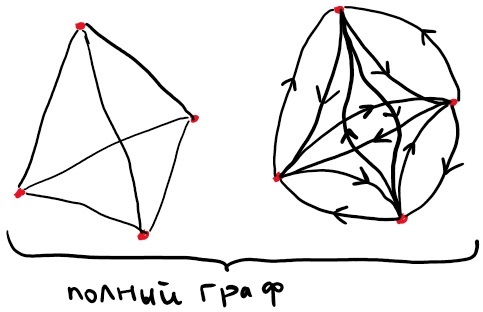
\includegraphics[width = 0.8\textwidth]{5.1}
	\small
	\begin{tcolorbox}[colframe=gray!50!black, left=5pt, right=5pt, top=5pt, bottom=5pt, boxrule=1pt, colback=gray!10!white]
		\begin {itemize}
		\item Еще есть "турнир" (Tournament) - это ориентированный простой граф, в котором между каждой парой разлиных вершин ровно 1 ребро\\
		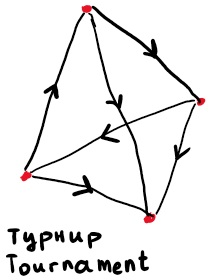
\includegraphics[width = 0.4\textwidth]{5.2}
	\end{itemize}
	\end{tcolorbox}
	\normalsize
\end{document}